\documentclass[11pt]{article}
\usepackage{url}
\usepackage{graphicx}
\usepackage{hyperref}
%\usepackage{latexsym,amssymb}
%\usepackage{amssymb,amsmath}

\usepackage[utf8]{inputenc}

% Default fixed font does not support bold face
\DeclareFixedFont{\ttb}{T1}{txtt}{bx}{n}{12} % for bold
\DeclareFixedFont{\ttm}{T1}{txtt}{m}{n}{12}  % for normal

% Custom colors
\usepackage{color}
\input{../../vrac/rgb.tex}

\usepackage{listings}

\newcommand\digitstyle{\color{deepgreen}}
\makeatletter
\newcommand{\ProcessDigit}[1]
{%
  \ifnum\lst@mode=\lst@Pmode\relax%
   {\digitstyle #1}%
  \else
    #1%
  \fi
}
\makeatother
\lstset{
}


\definecolor{deepblue}{rgb}{0,0,0.5}
\definecolor{deepred}{rgb}{0.6,0,0}
\definecolor{deepgreen}{rgb}{0,0.5,0}
\definecolor{MyLightGray}{rgb}{0.93,0.93,0.93}
\definecolor{MyPurple}{rgb}{.8,0,.8}
\definecolor{MyOrange}{rgb}{.8,0.4,0}


% Python style for highlighting
\newcommand\pythonstyle{\lstset{
literate=
    {0}{{{\ProcessDigit{0}}}}1
    {1}{{{\ProcessDigit{1}}}}1
    {2}{{{\ProcessDigit{2}}}}1
    {3}{{{\ProcessDigit{3}}}}1
    {4}{{{\ProcessDigit{4}}}}1
    {5}{{{\ProcessDigit{5}}}}1
    {6}{{{\ProcessDigit{6}}}}1
    {7}{{{\ProcessDigit{7}}}}1
    {8}{{{\ProcessDigit{8}}}}1
    {9}{{{\ProcessDigit{9}}}}1
    {<=}{{\(\leq\)}}1,
    morestring=[b]",
    morestring=[b]',
    morecomment=[l]//,
backgroundcolor=\color{MyLightGray},
language=Python,
basicstyle=\ttm,
morekeywords={self, {1}},              % Add keywords here
%keywordstyle=\ttb\color{deepblue},
%keywordstyle=\ttb\color{MyOrange},
keywordstyle=\color{MyOrange},
emph={as, import},          % Custom highlighting
%emphstyle=\ttb\color{deepred},    % Custom highlighting style
%emphstyle=\ttb\color{MyPurple},
emphstyle=\color{MyPurple},
stringstyle=\color{deepgreen},
frame=tb,                         % Any extra options here
showstringspaces=false
}}

% Python style for highlighting
\newcommand\outputstyle{\lstset{
%backgroundcolor=\color{MyLightGray},
language=Python,
basicstyle=\ttm,
%morekeywords={self, {1}},              % Add keywords here
%keywordstyle=\ttb\color{deepblue},
%keywordstyle=\ttb\color{MyOrange},
%keywordstyle=\color{MyOrange},
%emph={as, import},          % Custom highlighting
%emphstyle=\ttb\color{deepred},    % Custom highlighting style
%emphstyle=\ttb\color{MyPurple},
%emphstyle=\color{MyPurple},
%stringstyle=\color{deepgreen},
frame=tb,                         % Any extra options here
showstringspaces=false
}}



% Output environment
\lstnewenvironment{pythonoutput}[1][]
{
\outputstyle
\lstset{#1}
}
{}




% Python environment
\lstnewenvironment{python}[1][]
{
\pythonstyle
\lstset{#1}
}
{}

% Python for external files
\newcommand\pythonexternal[2][]{{
\pythonstyle
\lstinputlisting[#1]{#2}}}

% Python for inline
\newcommand\pythoninline[1]{{\pythonstyle\lstinline!#1!}}




\usepackage[english]{babel}
\usepackage{array}
\usepackage{multirow} 

\hypersetup{
pdfauthor={Julien Langou}, 
} 

\setlength{\oddsidemargin}{-0.5in}
\setlength{\evensidemargin}{-0.5in}

\setlength{\textwidth}{7.4in}
\setlength{\textheight}{10.0in}

\setlength{\topmargin}{-0.75in}
\setlength{\headheight}{0pt}
\setlength{\headsep}{0pt}

\setlength{\parindent}{0pt}

\begin{document}

\thispagestyle{empty}
\pagestyle{empty}
%\renewcommand{\theenumi}{\alph{enumi}}

%
%\framebox{
%\begin{minipage}{\textwidth}
%{\tiny
%{\bf Copyright (C) 2018, 2012, 2016 by Pearson Education Inc. All Rights Reserved,}
%please visit \url{www.pearsoned.com/permissions/}.}
%{\bf Copyright (C) 2018, 2012, 2016 by Pearson Education Inc. All Rights Reserved.}
%Printed in the United States of America.
%This publication is protected by copyright, and permission should be obatined from the 
%publisher prior to any prohibted reproduction, storage in retrieval system, or 
%transmission in any form of by any means, electronic, mechanical, photocopying, recording, 
%or otherwise. For information regarding permissions, request forms and the appropriate 
%contacts within the Pearson Education Global Rights \& Permissions department, 
%please visit \url{www.pearsoned.com/permissions/}.}
%
%\end{minipage}}

\framebox{
\begin{minipage}{\textwidth}
{\tiny
{\bf Copyright (c) 2021, Julien Langou. All rights reserved,}
please visit \url{https://creativecommons.org/licenses/by/4.0/}.}
\end{minipage}}
\vspace*{.2cm}

\framebox{
\begin{minipage}{\textwidth}
\textbf{EX.0.1.2.d Langou}\\\\
Let $p(x)$ be the polynomial
$$ p(x) = 5x^4 - 2x^3 + 3 x^2 - 9x + 7 $$
We want to evaluate $p(x)$ at $x=-1$ and $x=3$.\\
We will do it using 5 different methods.

\begin{enumerate}

\item Given $x$ as {\color{blue} \texttt{x}}, 
write a simple to expression to compute $p(x)$
the polynomial $p$ evaluated $x$,
as {\color{blue} \texttt{px}}.

\item
Given $x$ as {\color{blue} \texttt{x}},
using only statement of the form 
{\color{blue} \texttt{z =  z + c * x**i}}
write a sequence of statements that computes
{\color{blue} \texttt{z}} such that $z=p(x)$.
How many multiplications, additions, and power signs are you using?

\item
Given $x$ as {\color{blue} \texttt{x}},
incrementally compute the powers of $x$ with statements
of the form {\color{blue} \texttt{y~=~y~*~x}} 
(so that $y = x$, then $y = x^2$, then $y = x^3$, 
then $y = x^4$, etc.), then using only statement of the form 
{\color{blue} \texttt{z~=~z~+~c~*~y}},
write a sequence of statements that computes 
{\color{blue} \texttt{z}} such that $z=p(x)$
by avoiding the {\color{blue} \texttt{**}} power operator.
How many multiplications, additions, and power signs are you using?

\item Rewrite the polynomial $p(x)$ in nested form. 

\item Given $x$ as {\color{blue} \texttt{x}},
using only statement of the form 
{\color{blue}
\texttt{y = y * x + c}}, write a sequence of statements that computes 
{\color{blue} \texttt{y}} such that $y=p(x)$.
How many multiplications, additions, and power signs are you using?


\end{enumerate}
\end{minipage}}

\vspace*{.7cm}

\framebox{
\begin{minipage}{\textwidth}
{\tiny
{\bf Copyright (c) 2021, Julien Langou. All rights reserved,}
please visit \url{https://creativecommons.org/licenses/by/4.0/}.}
\end{minipage}}
\vspace*{.2cm}

\textbf{EX.0.1.2.d, Langou, solution, Langou}\\

See as well the {\color{red}\href{https://colab.research.google.com/drive/1vyAaAppnwBfUOh03Gh8S0hzpTsbncS3d?usp=sharing}{Colaboratory Jupyter Notebook}}.\\


\vspace*{.2cm}


{\color{blue}
\framebox{
\begin{minipage}{\textwidth}
\begin{enumerate}
\setcounter{enumi}{0}
\item 
Given $x$ as {\color{black} \texttt{x}}, 
write a simple to expression to compute $p(x)$
the polynomial $p$ evaluated $x$,
as {\color{black} \texttt{px}}.
\end{enumerate}
\end{minipage}}}
\vspace*{.2cm}

\begin{python}
import numpy as np

x = np.array( [ -1., 3. ])

px = 5. * x**4 - 2. * x**3 + 3. * x**2 - 9. * x + 7.

print( px )
\end{python}
\begin{pythonoutput}
[ 26. 358.]
\end{pythonoutput}

\vspace*{.2cm}

{\color{blue}
\framebox{
\begin{minipage}{\textwidth}
\begin{enumerate}
\setcounter{enumi}{1}
\item 
Given $x$ as {\color{black} \texttt{x}},
using only statement of the form 
{\color{black} \texttt{z =  z + c * x**i}}
write a sequence of statements that computes
{\color{black} \texttt{z}} such that $z=p(x)$.
How many multiplications, additions, and power signs are you using?
\end{enumerate}
\end{minipage}}}
\vspace*{.2cm}

\framebox{\begin{minipage}{0.20\textwidth}
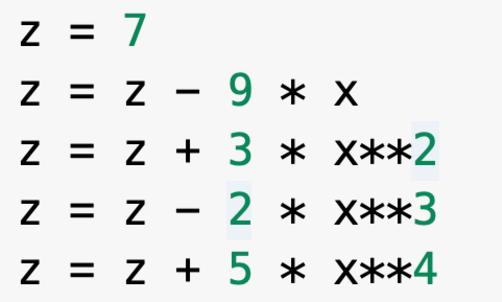
\includegraphics[width=\textwidth]{exercise_ex_0_1_02d__oer__langou___sol_langou___pdf1.pdf}
\end{minipage}}

We are using 4 additions/substractions, 4 multiplications, and 3 power signs.

\vspace*{.2cm}
{\color{blue}
\framebox{
\begin{minipage}{\textwidth}
\begin{enumerate}
\setcounter{enumi}{2}
\item
Given $x$ as {\color{black} \texttt{x}},
incrementally compute the powers of $x$ with statements
of the form {\color{black} \texttt{y~=~y~*~x}} 
(so that $y = x$, then $y = x^2$, then $y = x^3$, 
then $y = x^4$, etc.), then using only statement of the form 
{\color{black} \texttt{z~=~z~+~c~*~y}},
write a sequence of statements that computes 
{\color{black} \texttt{z}} such that $z=p(x)$
by avoiding the {\color{black} \texttt{**}} power operator.
How many multiplications, additions, and power signs are you using?
\end{enumerate}
\end{minipage}}}


\framebox{\begin{minipage}{0.35\textwidth}
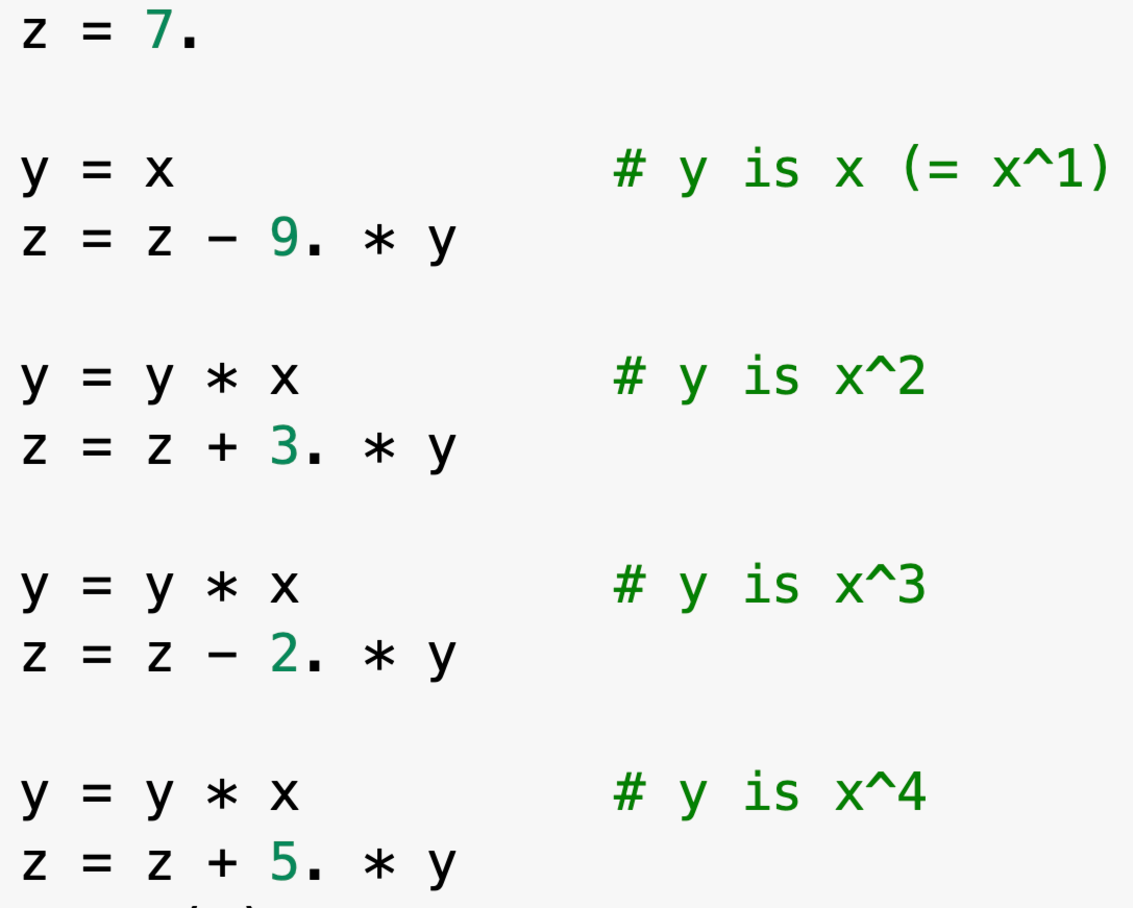
\includegraphics[width=\textwidth]{exercise_ex_0_1_02d__oer__langou___sol_langou___pdf6.pdf}
\end{minipage}}

We are using 4 additions/substractions, 7 multiplications, and 0 power signs.

\vspace*{.2cm}
{\color{blue}
\framebox{
\begin{minipage}{\textwidth}
\begin{enumerate}
\setcounter{enumi}{3}
\item Rewrite the polynomial $p(x)$ in nested form.
\end{enumerate}
\end{minipage}}}


\begin{eqnarray}
\nonumber p(x) & = & 5x^4 - 2x^3 + 3 x^2 - x + 7 \\
\nonumber      & = & ( ( ( 5 x - 2 ) x + 3 ) x - 1 ) x + 7
\end{eqnarray}


\framebox{\begin{minipage}{0.60\textwidth}

\includegraphics[width=\textwidth]{exercise_ex_0_1_02d__oer__langou___sol_langou___pdf5.pdf}
\end{minipage}}


\vspace*{.2cm}
{\color{blue}
\framebox{
\begin{minipage}{\textwidth}
\begin{enumerate}
\setcounter{enumi}{4}
\item
Given $x$ as {\color{black} \texttt{x}},
using only statement of the form 
{\color{black}
\texttt{y = y * x + c}}, write a sequence of statements that computes 
{\color{black} \texttt{y}} such that $y=p(x)$.
How many multiplications, additions, and power signs are you using?
\end{enumerate}
\end{minipage}}}
\vspace*{.2cm}


\framebox{\begin{minipage}{0.20\textwidth}
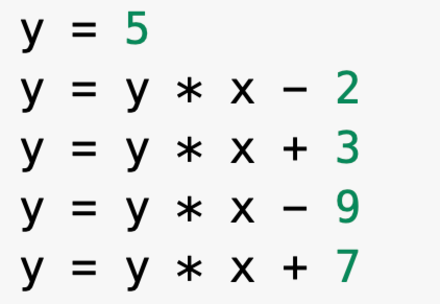
\includegraphics[width=\textwidth]{exercise_ex_0_1_02d__oer__langou___sol_langou___pdf2.pdf}
\end{minipage}}

We are using 4 additions/substractions, 4 multiplications, and 0 power signs.

\newpage
\vspace*{.2cm}
{\color{blue}
\framebox{
\begin{minipage}{\textwidth}
\begin{enumerate}
\setcounter{enumi}{3}
\item
(python) Using Python, evaluate with and without nested form at $x=-1$ and $x=3$.
\end{enumerate}
\end{minipage}}}
\vspace*{.2cm}


\framebox{\begin{minipage}{0.80\textwidth}
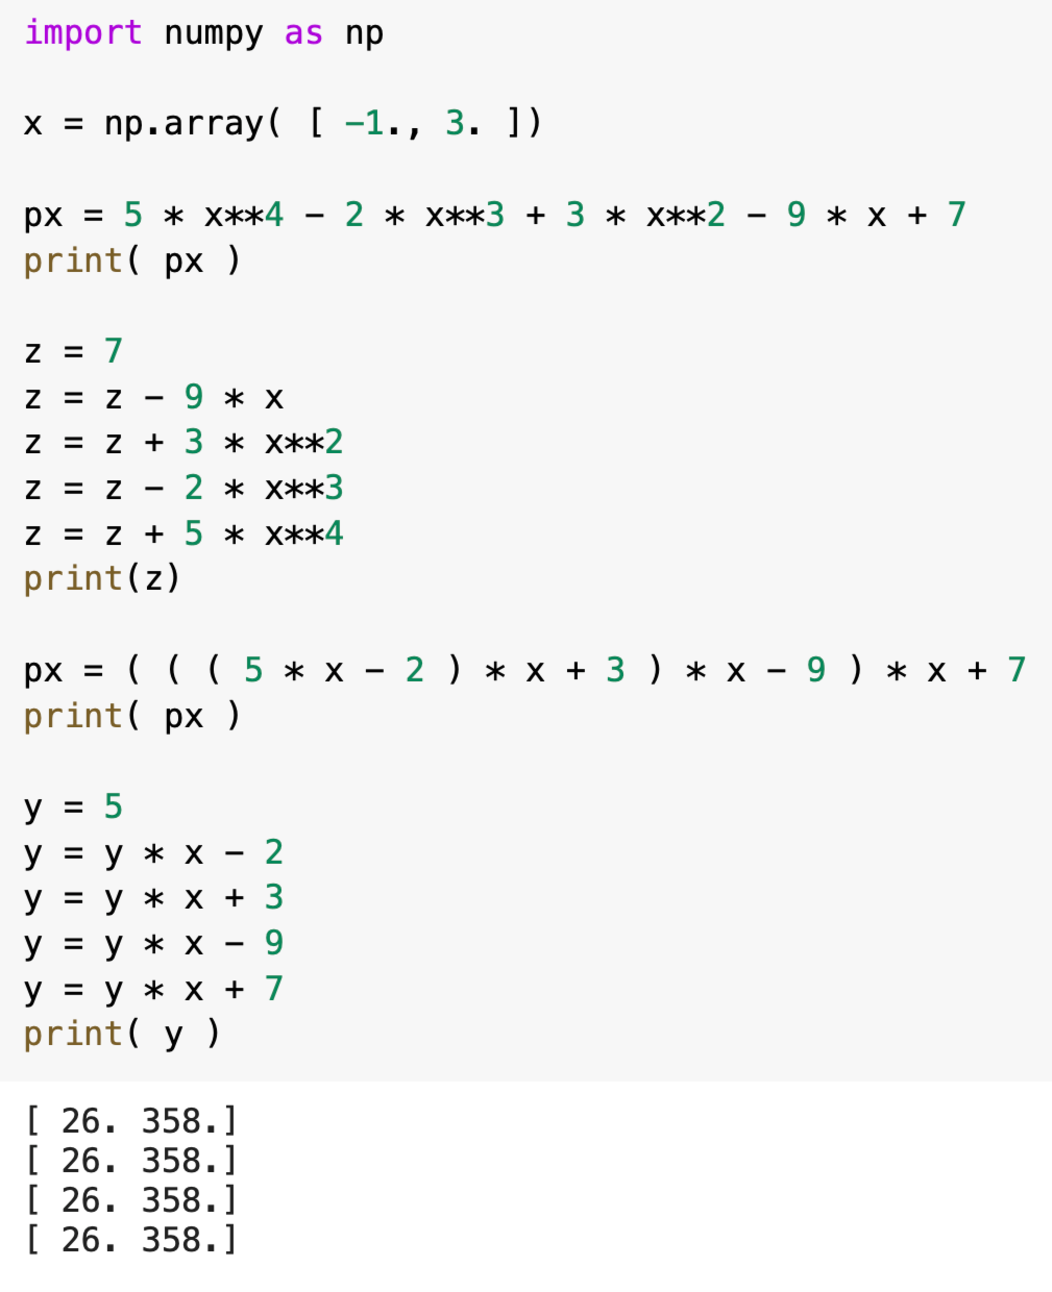
\includegraphics[width=\textwidth]{exercise_ex_0_1_02d__oer__langou___sol_langou___pdf3.pdf}
\end{minipage}}





\end{document}
